\section{Circuitos RLC}

\frame{
	\frametitle{Introdução}
	\begin{block}{Introdução}
		Conhecidos os elementos $R$, $L$ e $C$ e suas relações de corrente e tensão, podemos agora analisar o caso em que a força eletromotriz alternada é aplicada ao circuito RLC.
	\end{block}

	\medskip

	\setmyunit{2cm}
	\centering
	\begin{circuitikz}
		\draw (0,0) to[sV,l=$ v(t) $] ++(0,-1.5)
		to[C,l=$ C $] ++(1.5,0)
		to[L,l=$ L $] ++(0,1.5)
		(0,0) to[R,l=$ R $] ++(1.5,0);
	\end{circuitikz}
%	\centerline{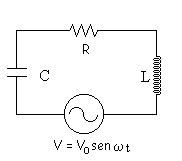
\includegraphics[width=0.4\linewidth]{Figuras/Ch14/rlc.png}}
}

\frame{
	\frametitle{Revisão}
	\begin{block}{Lembrando...}
		\begin{itemize}
			\item \textbf{Resistor:} a corrente e a tensão estão em fases.
			\item \textbf{Capacitor:} a corrente está adiantada de $\ang{90}$ da tensão.
			\item \textbf{Indutor:} a corrente está atrasada de $\ang{90}$ da tensão.
		\end{itemize}
	\end{block}
}

\frame{
	\frametitle{Lei das tensões de Kirchhoff para C.A.}

	\setmyunit{2cm}
	\centering
	\begin{circuitikz}
		\draw (0,0) to[sV,l=$ v(t) $] ++(0,-1.5)
		to[C,l=$ C $] ++(1.5,0)
		to[L,l=$ L $] ++(0,1.5)
		(0,0) to[R,l=$ R $] ++(1.5,0);
	\end{circuitikz}

	\begin{block}{Soma vetorial}
		Lembrando que devido as defasagens angulares, a LKT deve ser aplicada utilizando uma soma vetorial, e não algébrica. Deste modo,
		$$\vec{V} = \vec{V_R} + \vec{V_L} + \vec{V_C}$$
	\end{block}
}

\frame{
	\frametitle{Relação entre $\vec{V_L}$ e $\vec{V_C}$ }
	\setmyunit{1.5cm}
	\centering
	\begin{tikzpicture}
		\draw[->] (0,-0.7) -- (0,1.2) node[above] {$ y $};
		\draw[->] (-0.2,0) -- (1.7,0) node[right] {$ x $};
		
		\draw[-Latex,blue] (0,0) -- node[below] {$ \vec{V_R} $} (1.5,0);
		\draw[-Latex,red] (0,0) -- node[below] {$ i $} (0.5,0);
		
		\draw[-Latex,blue] (0,0) -- (0,1) node[right] {$ \vec{V_L} $};
		\draw[-Latex,black!60!blue] (0,0) -- (0,0.5) node[left] {$ |\vec{V_L}|-|\vec{V_C}| $};
		\draw[-Latex,blue] (0,0) -- (0,-0.5) node[right] {$ \vec{V_C} $};
		
		\draw[-Latex] (0,0) -- (1.5,0.5) node[above] {$ \vec{V_F} $};
		
		\draw[dashed] (0,0.5) -- (1.5,0.5) -- (1.5,0);
		
		\coordinate (O) at (0,0);
		\coordinate (A) at (1,0);
		\coordinate (B) at (1.5,0.5);
		
		\pic[draw, angle radius=25pt,angle eccentricity=1,"$ \theta $" {xshift=4pt,yshift=1pt}] {angle=A--O--B};
		
		\node[coordinate] (C) at (2,0.8) {};
		\draw[-stealth] (C) edge[bend right] node[above right] {$\omega$} +(-0.25,0.25);
	\end{tikzpicture}
	
%	\centerline{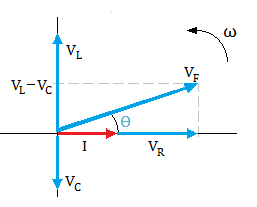
\includegraphics[width=0.4\linewidth]{Figuras/Ch14/vet2rlc.png}}

	\begin{block}{Soma vetorial}
		Como os vetores $\vec{V_L}$ e $\vec{V_C}$ têm a mesma direção e sentidos opostos, podemos simplificar a soma vetorial combinando $\vec{V_L}$ e $\vec{V_C}$ para formar o vetor $\vec{V_L + V_C}$
	\end{block}
}

\frame{
	\frametitle{Tensão em um circuito RLC}
	\setmyunit{1.5cm}
	\centering
	\begin{tikzpicture}
	\draw[->] (0,-0.7) -- (0,1.2) node[above] {$ y $};
	\draw[->] (-0.2,0) -- (1.7,0) node[right] {$ x $};
	
	\draw[-Latex,blue] (0,0) -- node[below] {$ \vec{V_R} $} (1.5,0);
	\draw[-Latex,red] (0,0) -- node[below] {$ i $} (0.5,0);
	
	\draw[-Latex,blue] (0,0) -- (0,1) node[right] {$ \vec{V_L} $};
	\draw[-Latex,black!60!blue] (0,0) -- (0,0.5) node[left] {$ |\vec{V_L}|-|\vec{V_C}| $};
	\draw[-Latex,blue] (0,0) -- (0,-0.5) node[right] {$ \vec{V_C} $};
	
	\draw[-Latex] (0,0) -- (1.5,0.5) node[above] {$ \vec{V_F} $};
	
	\draw[dashed] (0,0.5) -- (1.5,0.5) -- (1.5,0);
	
	\coordinate (O) at (0,0);
	\coordinate (A) at (1,0);
	\coordinate (B) at (1.5,0.5);
	
	\pic[draw, angle radius=25pt,angle eccentricity=1,"$ \theta $" {xshift=4pt,yshift=1pt}] {angle=A--O--B};
	
	\node[coordinate] (C) at (2,0.8) {};
	\draw[-stealth] (C) edge[bend right] node[above right] {$\omega$} +(-0.25,0.25);
	\end{tikzpicture}
	
%	\centerline{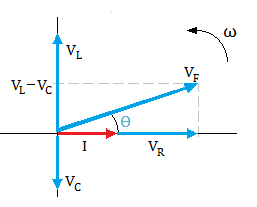
\includegraphics[width=0.4\linewidth]{Figuras/Ch14/vet2rlc.png}}

	\bigskip
	
	\begin{block}{Aplicando o Teorema de Pitágoras...}
		$$|\vec{V_F}|^2 = |\vec{V_R}|^2 + (|\vec{V_L}| - |\vec{V_C}|)^2$$
	\end{block}
}

\frame{
	\frametitle{Relação entre as impedâncias}
	\setmyunit{1.5cm}
	\centering
	\begin{tikzpicture}
	\draw[->] (0,-0.7) -- (0,1.2) node[above] {$ y $};
	\draw[->] (-0.2,0) -- (1.7,0) node[right] {$ x $};
	
	\draw[-Latex,blue] (0,0) -- node[below] {$ \vec{R} $} (1.5,0);
%	\draw[-Latex,red] (0,0) -- node[below] {$ i $} (0.5,0);
	
	\draw[-Latex,blue] (0,0) -- (0,1) node[right] {$ \vec{X_L} $};
	\draw[-Latex,black!60!blue] (0,0) -- (0,0.5) node[left] {$ |\vec{X_L}|-|\vec{X_C}| $};
	\draw[-Latex,blue] (0,0) -- (0,-0.5) node[right] {$ \vec{X_C} $};
	
	\draw[-Latex] (0,0) -- (1.5,0.5) node[above] {$ \vec{Z} $};
	
	\draw[dashed] (0,0.5) -- (1.5,0.5) -- (1.5,0);
	
	\coordinate (O) at (0,0);
	\coordinate (A) at (1,0);
	\coordinate (B) at (1.5,0.5);
	
	\pic[draw, angle radius=25pt,angle eccentricity=1,"$ \theta $" {xshift=4pt,yshift=1pt}] {angle=A--O--B};
	
	\node[coordinate] (C) at (2,0.8) {};
	\draw[-stealth] (C) edge[bend right] node[above right] {$\omega$} +(-0.25,0.25);
	\end{tikzpicture}
	
%	\centerline{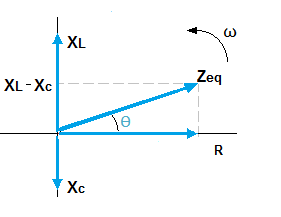
\includegraphics[width=0.4\linewidth]{Figuras/Ch14/vetrlc.png}}
	\begin{block}{Soma vetorial}
		Dividindo os vetores $\vec{V}$ pelo referencial $i$, tem-se um novo diagrama, agora de oposições.
		
		\begin{gather*}
			|\vec{Z}|^2 = |\vec{R}|^2 + (|\vec{X_L}| - |\vec{X_C}|)^2\\[0.5em]
			\phi = \arctg \Big(\dfrac{|\vec{X_L}| - |\vec{X_C}|}{|\vec{R}|} \Big)
		\end{gather*}
	\end{block}
}

\frame{
	\frametitle{Constante de fase $\phi$}
	\begin{block}{Temos três casos, dependendo dos valores de $|\vec{X_L}|$ e $|\vec{X_C}|$}
		\begin{itemize}
			\item $|\vec{X_L}| > |\vec{X_C}|$: o circuito é mais indutivo que capacitivo. Neste caso $\phi > 0$ e $i$ está atrasado em relação a $v(t)$. \vspace{0.5cm}
			\item $|\vec{X_C}| > |\vec{X_L}|$: o circuito é mais capacitivo que indutivo. Neste caso $\phi < 0$ e $i$ está adiantado em relação a $v(t)$. \vspace{0.5cm}
			\item $|\vec{X_C}| = |\vec{X_L}|$: o circuito está em ressonância. Neste caso $\phi = 0$ e $i$ está em fase em relação a $v(t)$. \vspace{0.5cm}
		\end{itemize}
	\end{block}
}

\frame{
	\frametitle{Ressonância}
	\begin{block}{Definição}
		O diagrama das tensões de um circuito RLC série resulta em um triângulo retângulo cujo
		cateto oposto a $\phi$ é $|\vec{V_L}| - |\vec{V_C}|$.
		
		\vspace{0.5cm}
		O caso particular em que esse cateto é nulo $(|\vec{V_L}| - |\vec{V_C}| = 0)$, isto é $|\vec{V_L}| = |\vec{V_C}|$, tem
		aplicações práticas importantes, e o circuito que apresenta essa característica é chamado circuito em ressonância ou \textbf{circuito ressonante}.
		
		\vspace{0.5cm}
		Nesse caso, toda a energia reativa é trocada entre o indutor e o capacitor, e a fonte fornece
		apenas a energia para o resistor. Para a fonte, o circuito é resistivo puro.
	\end{block}
}

\frame{
	\frametitle{Frequência de Ressonância}
	\begin{block}{Evolução de $\vec{X_L}$ e $\vec{X_C}$ com o tempo}
		\begin{itemize}
			\item \textbf{Caso 1:} Quando a frequência $\omega$ é pequena. \\

			      \begin{itemize}
				      \item \normalsize A reatância $(|\vec{X_L}|=\omega L)$ é pequena.
				      \item \normalsize A reatância $(|\vec{X_C}|=1/\omega C)$ é grande.
				      \item \normalsize O circuito é principalmente capacitivo, o que mantém a corrente baixa.
			      \end{itemize}
		\end{itemize}
		$$i = \dfrac{U}{\sqrt{|\vec{R}|^2 + (|\vec{X_L}| - |\vec{X_C}|)^2}}$$
	\end{block}
}

\frame{
	\frametitle{Frequência de Ressonância}
	\begin{block}{Evolução de $\vec{X_L}$ e $\vec{X_C}$ com o tempo}
		\begin{itemize}
			\item \textbf{Caso 2:} Quando a frequência $\omega$ aumenta.
			
			\begin{itemize}
				\item \normalsize A reatância $(|\vec{X_L}|=\omega L)$ começa a aumentar.
				\item \normalsize A reatância $(|\vec{X_C}|=1/\omega C)$ continua ser dominante, mas diminui.
				\item \normalsize A impedância começa a diminuir, o que faz a corrente aumentar.
			\end{itemize}
		\end{itemize}
		$$i = \dfrac{U}{\sqrt{|\vec{R}|^2 + (|\vec{X_L}| - |\vec{X_C}|)^2}}$$
	\end{block}
}

\frame{
	\frametitle{Frequência de Ressonância}
	\begin{block}{Evolução de $\vec{X_L}$ e $\vec{X_C}$ com o tempo}
		\begin{itemize}
			\item \textbf{Caso 3:} Quando a frequência $\omega$ aumenta tal que $|\vec{X_L}| = |\vec{X_C}|$
			      \begin{itemize}
				      \item \normalsize A corrente atinge o valor máximo.
				      \item \normalsize O circuito está em ressonância.
			      \end{itemize}
		\end{itemize}
		$$|\vec{X_L}| = |\vec{X_C}| \implies \omega L = \dfrac{1}{\omega C} \implies \omega = \dfrac{1}{\sqrt{LC}}$$
	\end{block}
}

\frame{
	\frametitle{Frequência de Ressonância}
	\begin{block}{Evolução de $\vec{X_L}$ e $\vec{X_C}$ com o tempo}
		\begin{itemize}
			\item \textbf{Caso 4:} Quando a frequência $\omega$ aumenta mais ainda.

			      \begin{itemize}
				      \item \normalsize A reatância $(|\vec{X_L}| =\omega L)$ é predominante.
				      \item \normalsize A reatância $(|\vec{X_C}| =1/\omega C)$ diminui.
				      \item \normalsize A impedância começa a aumentar, o que faz a corrente dimninuir.
			      \end{itemize}
		\end{itemize}
		$$i = \dfrac{U}{\sqrt{|\vec{R}|^2 + (|\vec{X_L}| - |\vec{X_C}|)^2}}$$
	\end{block}
}

\frame{
	\frametitle{Frequência de Ressonância}
	\centerline{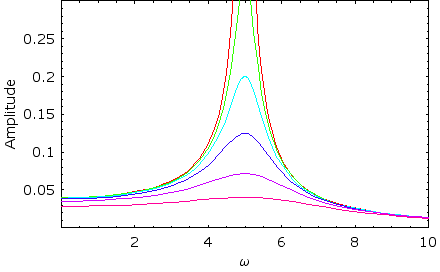
\includegraphics[width=1.0\linewidth]{Figuras/Ch14/ressonancia.png}}
}

\frame{
	\frametitle{Exemplo}
	\begin{block}{}
		01. Considere um circuito RLC série com $R = \SI{1}{\ohm} , L = \SI{10}{\milli\henry}$ e $C$ desconhecido. Qual o valor de $C$ necessário para que este circuito sintonize na frequência $f = \SI{150}{\kilo\hertz}$?
		
		\vspace{1cm}
		\textbf{Solução:}
		\begin{gather*}
			\omega = \dfrac{1}{\sqrt{LC}} \implies 2\pi f = \dfrac{1}{\sqrt{LC}}\\
			2\pi \times \num{150e3} = \dfrac{1}{\sqrt{ \num{10e-3} C}} \implies C = \SI{112.6}{\pico\farad}
		\end{gather*}
	\end{block}
}

\section*{Exercícios}

\frame{
	\frametitle{Exercícios}
	\begin{block}{}
		01. Num circuito RLC série, a tensão eficaz no resistor, indutor e capacitor valem, respectivamente, \SI{30}{\volt}, \SI{90}{\volt} e \SI{50}{\volt}. Determine o valor da tensão eficaz da fonte C.A. que alimenta o circuito.

		\vspace{0.3cm}

		02. Qual a frequência de ressonância de um circuito RLC série, se $R = \SI{1}{\milli\ohm}$, $L = \SI{1}{\milli\henry}$ e $C = \SI{1}{\milli\farad}$?

		\vspace{0.3cm}

		03. Verificar se o circuito abaixo é capacitivo, indutivo, ou resistivo, dados: $ v(t)=40\sen(100t+\ang{20}) $, $ C=\SI{1/16000}{\farad} $, $ L=\SI{2}{\henry} $ e $ R=\SI{60}{\ohm} $. Calcule ainda a impedância, a constante de fase $\phi$ e a corrente eficaz.
	\end{block}
%	\centerline{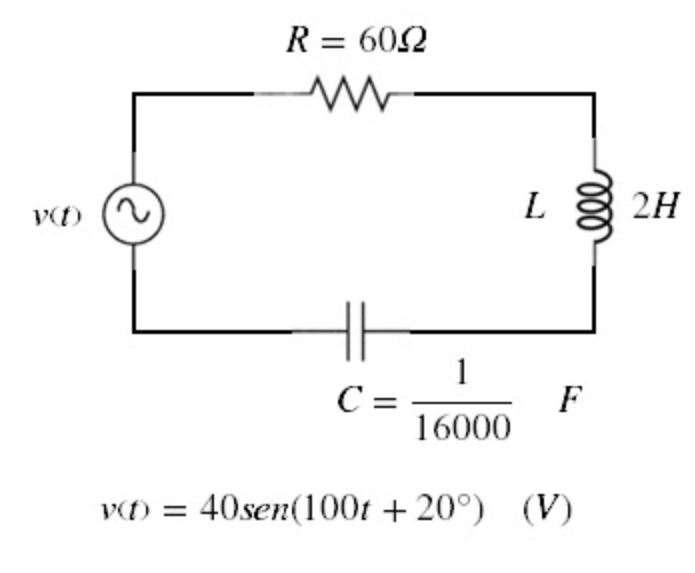
\includegraphics[width=0.4\linewidth]{Figuras/Ch14/ex03.PNG}}

\setmyunit{1.2cm}
\centering
\begin{circuitikz}
	\ctikzset{resistors/scale=0.5, capacitors/scale=0.5, sources/scale=0.6, inductors/scale=0.6}
	\draw (0,0) to[sV,l_=$ v(t) $] ++(0,-1.5)
	to[C,l=$ C $] ++(1.5,0)
	to[L,l_=$ L $] ++(0,1.5)
	(0,0) to[R,l=$ R $] ++(1.5,0);
\end{circuitikz}

}


\section*{Referências}

\frame{
	\frametitle{Referências e Exercícios Complementares}
	\begin{itemize}
		\item ALEXANDRE, Charles K.; SADIKU, Matthew N. O. Fundamentos de Circuitos Elétricos. 5. ed. Porto Alegre: AMGH, 2013.
	\end{itemize}
	%\centering{\alert{Página 36 - \textbf{1.6.1 até 1.6.5, 1.6.17 até 1.6.19}}} \\
	\centering{\alert{Lista de exercícios 14}}
}